\documentclass[10pt]{article}
\usepackage[a4paper,margin=2cm]{geometry}
\usepackage{booktabs,longtable,amsmath,amssymb,graphicx,pdfpages,caption,lscape}
\captionsetup{font=small,labelfont=bf}
\title{\bfseries CL inflow fits of the SPARC category-E galaxies:\\ poor single-L fits without detectable structure}
\author{Automated analysis for E.P.J.\ de Haas}\date{}
\begin{document}\maketitle
\section*{Summary}
Category E contains the 17 SPARC galaxies whose single-Lagrangian (single-L) fit has $\chi^2_\nu>1$ but whose residual signs pass the runs test ($p\ge0.05$): the fit is poor, yet no coherent pattern is detected. We show that this combination arises mainly because the curves are short (median $n=10$; 15 of 17 have $n\le13$). For $n=4$--5 the runs test cannot reach $p<0.05$ for \emph{any} sign sequence, and for $n\le13$ it detects only very clean patterns. Testing the model extensions directly by BIC, as for categories C and D ([1,2]), gives 11 galaxies in which an extension is strongly preferred ($\Delta\mathrm{BIC}<-6$). Of these, 5 show a \emph{rising window}, closely related to a Lagrangian reset (B-like; statistically equivalent in three), all in Im/Sm galaxies. 3 show a \emph{descent window} (C-like), in Sb--Sc spirals. 3 need two windows (D-like). The remaining 6 galaxies are adequately described by single-L with a modest intrinsic velocity scatter (median 2.1\,km\,s$^{-1}$), their excess $\chi^2$ dominated by a single point. Category E is therefore not a physically distinct class. It consists of B-, C- and D-type galaxies that the sign test could not recognise with few points, plus single-L galaxies with slightly underestimated errors. The morphological split of B (late types, reset) versus C (bulged spirals, descent) reappears here.

\section{Models and tests}
The same model set as for category D was used, with $X=\sqrt{2GM/R}-H_zR$, $Y(r)=\sqrt{2GM/r}-H_zr$, $H_z=2.2\times10^{-18}$\,s$^{-1}$, fits on $v^2$ with $\sigma_{v^2}=2V_\mathrm{obs}\delta V_\mathrm{obs}$:
\textbf{S} single-L [2, Eqs.~17--18] ($k=2$); \textbf{VW} one virial window [1, Eq.~6; 2, Eq.~19] with continuous gauge and descent-mass parametrisation $M_N=(p-2)M$ ($k=4$; $n\ge6$); \textbf{2L} two Lagrangians [2, Eqs.~24--26] ($k=4$; $n\ge6$); \textbf{VW2} two windows [1, Eqs.~5--7] ($k=6$; $n\ge10$). The preferred model has the lowest BIC (a simpler model within $\Delta\mathrm{BIC}<2$ is preferred), and an extension must beat S by $\Delta\mathrm{BIC}<-6$. Status as in the D report: \textbf{clean} (all parameters within 60\%, jackknife scatter within 60\%, at least 3 points on each side of the first window radius, no bound or $|p|>100$, $\chi^2_\nu\le2$), \textbf{weakly constrained} (one of these fails), \textbf{phenomenological} (bulge radius at bound or $|p|>100$).

\paragraph{Power of the runs test.} For $n$ residuals the smallest attainable one-sided runs-test $p$ is reached by two equal runs. It is 0.110 ($n=4$), 0.063 ($n=5$), 0.020 ($n=7$), 0.0036 ($n=10$) and $7\times10^{-4}$ ($n=13$). With 4--5 points no pattern can ever be significant. With 7--10 points only the cleanest two- or three-run sequences reach $p<0.05$, and a single misplaced sign is enough to fail.
\paragraph{Scatter and outlier tests on single-L.} (a) Intrinsic velocity scatter $\sigma_\mathrm{int}$, added in quadrature to $\delta V_\mathrm{obs}$ and refitted, such that $\chi^2_\nu=1$. (b) Influence of the worst point: $\chi^2_\nu$ after removing it and refitting. (c) Robust (soft-$\ell_1$) refit. (d) Upper-tail probability $P(\chi^2\ge\chi^2_\mathrm{obs})$. Distance and inclination systematics as in the A--D reports.

\section{Outcome}
\begin{table}[h]\centering\small\caption{Category-E outcome by preferred description.}\begin{tabular}{llp{10cm}}\toprule Preferred description & $N$ & Galaxies (type, $n$, status)\\\midrule
rising window (B-like) & 5 & UGC05716 (Sm, 12, clean), UGC11820 (Sm, 10, clean), ESO444--G084 (Im, 7, weakly constrained), UGC00191 (Sm, 9, weakly constrained), DDO168 (Im, 10, weakly constrained)\\
descent window (C-like) & 3 & NGC0801 (Sc, 13, clean), NGC2683 (Sb, 11, weakly constrained), NGC2998 (Sc, 13, weakly constrained)\\
two windows (D-like) & 3 & NGC2955 (Sb, 24, phenomenological), NGC6195 (Sb, 23, weakly constrained), UGC05764 (Im, 10, weakly constrained)\\
single-L kept & 6 & NGC3893 (Sc, 10, single-L kept), NGC4051 (Sbc, 7, single-L kept), UGC00634 (Sm, 4, single-L kept), UGC00891 (Sm, 5, single-L kept), UGC02455 (Im, 8, single-L kept), UGCA442 (Sm, 8, single-L kept)\\
\bottomrule\end{tabular}\end{table}
\begin{figure}[h]\centering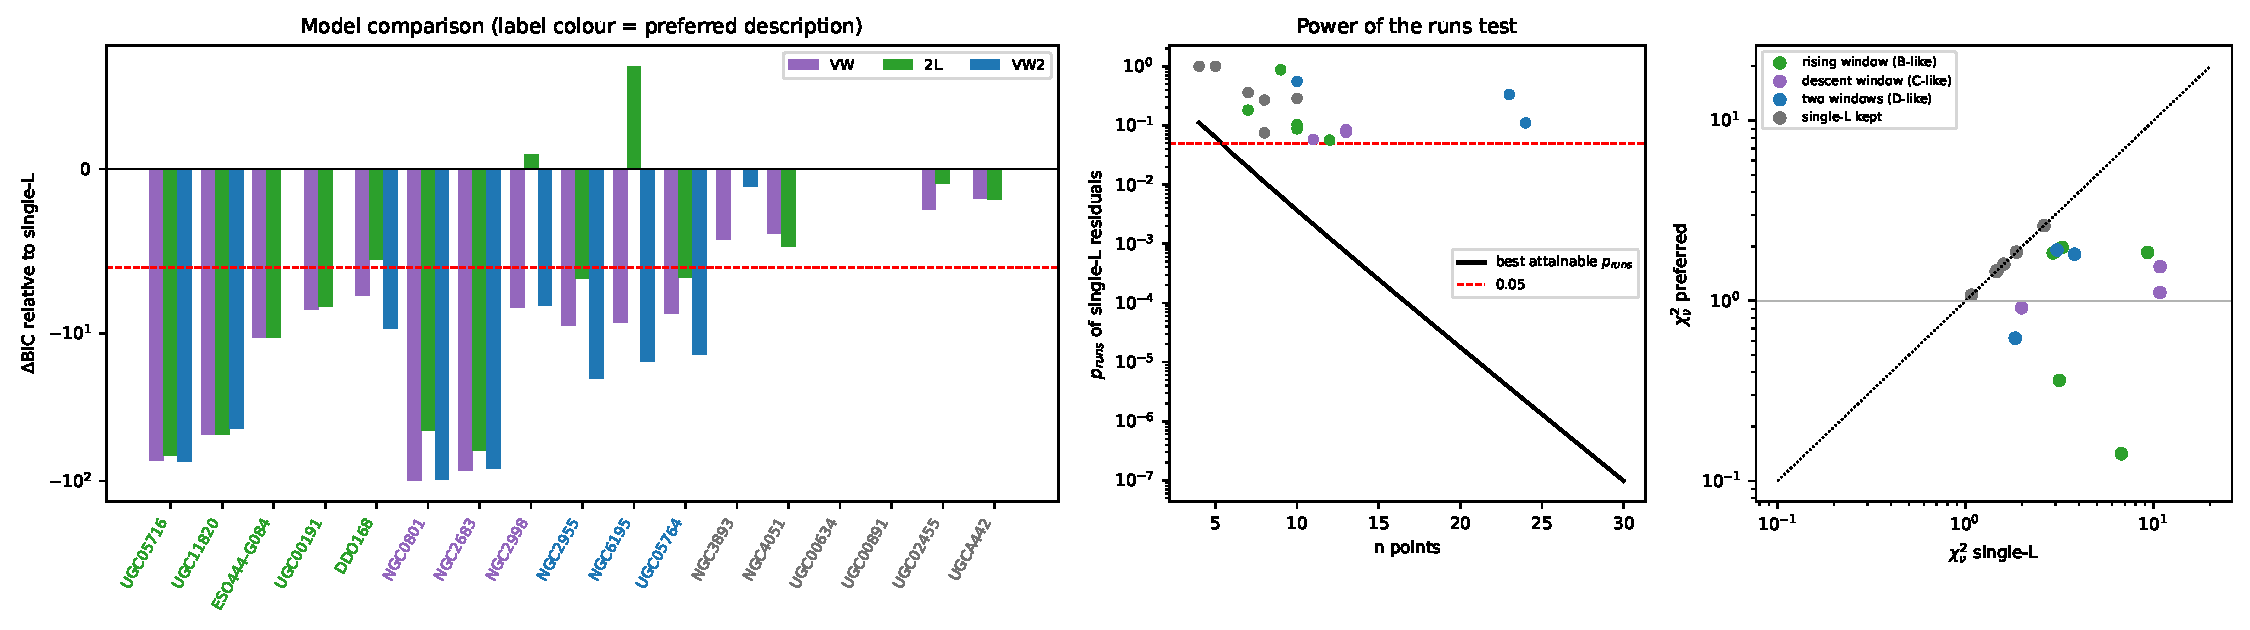
\includegraphics[width=\textwidth]{catE_fig_models.pdf}\caption{Left: $\Delta$BIC of each extension relative to single-L (red: $-6$); label colour = preferred description (green rising window, purple descent, blue two windows, grey single-L). Middle: runs-test $p$ of the single-L residuals versus $n$, with the best attainable $p$ (black) and the 0.05 level; for small $n$ no or only very clean patterns can be detected. Right: $\chi^2_\nu$ single-L versus preferred model.}\end{figure}
\paragraph{Rising windows, B-like (5).} DDO168, ESO444--G084, UGC00191, UGC05716, UGC11820, all Im/Sm with 7--12 points. Beyond $r_v\approx1.1$--6.3\,kpc the curve rises above the single-L continuation ($p<0$). In ESO444-G084, UGC 191 and UGC 11820 two-L is statistically equivalent ($|\mathrm{BIC_{2L}-BIC_{VW}}|<0.3$); DDO 168 and UGC 5716 prefer the window by 2.2 and 5.8. They are the short-curve counterparts of the category-B nested-spiral galaxies. UGC 5716 and UGC 11820 are clean (single-L $\chi^2_\nu$ 9.3 and 6.7 $\to$ 1.85 and 0.14). The other three have too few points before $r_v$ for stable parameters.

\paragraph{Descent windows, C-like (3).} NGC 801 (Sc), NGC 2683 (Sb) and NGC 2998 (Sc): $\chi^2_\nu$ 10.8, 10.8 and 2.0 $\to$ 1.5, 1.1 and 0.9, with $\Delta\mathrm{BIC}=-100$, $-85$ and $-8$. NGC 801 is clean ($r_v=4.2$\,kpc, $p=3.5$, close to the pure Kepler case). In NGC 2683 only two points precede the window, and in NGC 2998 the descent rests on the last two points, so both are weakly constrained. The two edge-on systems (NGC 801, NGC 2683; $i=80^\circ$) have the largest single-L $\chi^2_\nu$ of the category.

\paragraph{Two windows, D-like (3).} NGC 6195 (Sb) is well fitted by a near-Kepler descent ($p\approx3$) followed by a flattening ($q\approx0.6$), but has only two points inside the first window radius. UGC 5764 (Im) is improved but its parameters are unstable. NGC 2955 (Sb) is phenomenological ($|q|>100$, parameter uncertainties $\gg100$\%), like the bulge-dominated D galaxies.

\paragraph{Single-L kept (6).} NGC3893, NGC4051, UGC00634, UGC00891, UGC02455, UGCA442. No extension is justified. Their excess $\chi^2$ is small (single-L $\chi^2_\nu$ 1.07--2.61; upper-tail $P(\chi^2\ge\chi^2_\mathrm{obs})$ from 0.023 to 0.36) and is dominated by one point: removing the worst point gives $\chi^2_\nu$ = 0.65--1.18. An intrinsic scatter of 0.2--10.4\,km\,s$^{-1}$ (median 2.1, i.e.\ 3\% of the median speed) brings $\chi^2_\nu$ to 1. That level is typical of non-circular motions and is consistent with single-L describing these galaxies as well as it describes category A.
\section{Fit quality and robustness}
\begin{table}[h]\centering\small\caption{Fit-quality statistics (medians, single-L $\to$ preferred).}\begin{tabular}{lrrrr}\toprule & Rising (5) & Descent (3) & Two windows (3) & Single-L kept (6)\\\midrule
$\chi^2_\nu$ & 3.26 $\to$ 1.84 & 10.79 $\to$ 1.11 & 3.06 $\to$ 1.81 & 1.53 $\to$ 1.53\\
RMS$_\mathrm{rel}$ & 0.235 $\to$ 0.109 & 0.250 $\to$ 0.088 & 0.121 $\to$ 0.039 & 0.171 $\to$ 0.171\\
$n$ & 10 & 13 & 23 & 7\\
$\sigma_\mathrm{int}$ (km/s, single-L) & 2.3 & 18.0 & 5.1 & 2.1\\
\bottomrule\end{tabular}\end{table}
None of the preferred fits leaves residual sign structure ($p_\mathrm{runs}\ge0.05$ in all cases), but with this few points that criterion is weak, as shown above. The single-L parameters are robust against the treatment of the excess scatter: the robust (soft-$\ell_1$) refit changes $M$ and $R$ by a median 2\% and 1\%, and inflating the errors by $\sigma_\mathrm{int}$ changes them by 5\% and 2\%. Hence the single-L scales of category E can be used, provided their errors are scaled by $\sqrt{\chi^2_\nu}$ or $\sigma_\mathrm{int}$ is included. For the accepted extensions the parameter precision is limited by the number of points on either side of the window radius. Only NGC 801, UGC 5716 and UGC 11820 meet the clean criteria.
\section{Assessment}
\begin{enumerate}\itemsep1pt
\item \textbf{Category E is a low-power class, not a physical one.} Poor fits without detected structure occur because the runs test has little power for $n\lesssim13$. When the extensions of [1,2] are tested directly by BIC, 11 of 17 galaxies are described by the same features as categories B, C and D.
\item \textbf{The B/C morphological split holds.} The rising (reset-like) windows occur in Im/Sm galaxies, and the descents in Sb--Sc spirals, as in categories B and C.
\item \textbf{The rest are single-L galaxies with a few km/s of extra scatter.} 6 galaxies need no extension. Their excess $\chi^2$ is carried by single points and corresponds to $\sigma_\mathrm{int}\approx2$\,km\,s$^{-1}$.
\item \textbf{Pipeline consequence.} For short curves the sign-based screen should be replaced or complemented by the direct BIC comparison of the extensions, with $n\le13$ results flagged as tentative. Applied to all 175 galaxies, this would merge category E into A--D.
\end{enumerate}

\section*{References}\small
[1] E.P.J.\ de Haas (2026), From Rotation Curves to Cosmic Time: Probing High-Redshift Expansion through Nested Spiral Dynamics, \emph{J.\ High Energy Phys.\ Grav.\ Cosmol.} 12, 334--367, doi:10.4236/jhepgc.2026.121022 (virial term Eq.~3; multi-region virial model Eqs.~5--7).\par
[2] E.P.J.\ de Haas, Galactic Rotation Curves and the Constant--Lagrangian Field: Empirical Tests within the $Q_g$ Rotor Framework (manuscript; single-L Eqs.~17--18, virial term Eq.~19, two-L Eqs.~24--26).\par
[3] F.\ Lelli, S.S.\ McGaugh, J.M.\ Schombert (2016), SPARC, \emph{AJ} 152, 157.

\clearpage\begin{landscape}{\scriptsize\setlength{\tabcolsep}{3pt}
\begin{longtable}{lllrrlrrrrrrrrl}
\caption{All category-E galaxies: single-L fit, scatter diagnostics and model comparison ($\Delta$BIC relative to single-L; -- = not fitted).}\\\toprule
Galaxy & Type & Q & $i$ & $n$ & signs & $p_\mathrm{runs}$ & $p_\mathrm{min}$ & $\chi^2_{\nu,S}$ & $\sigma_\mathrm{int}$ & $\chi^2_{\nu,-1}$ & VW & 2L & VW2 & preferred / status\\\midrule\endfirsthead
\toprule Galaxy & Type & Q & $i$ & $n$ & signs & $p_\mathrm{runs}$ & $p_\mathrm{min}$ & $\chi^2_{\nu,S}$ & $\sigma_\mathrm{int}$ & $\chi^2_{\nu,-1}$ & VW & 2L & VW2 & preferred / status\\\midrule\endhead\bottomrule\endfoot
UGC05716 & Sm & 2 & 54 & 12 & \texttt{+++--+++++++} & 0.056 & 0.001 & 9.28 & 3.6 & 6.21 & -73.0 & -67.2 & -74.3 & one window / clean\\
UGC11820 & Sm & 1 & 45 & 10 & \texttt{++++++--++} & 0.087 & 0.004 & 6.72 & 9.6 & 4.89 & -48.3 & -48.3 & -43.9 & one window / clean\\
ESO444--G084 & Im & 2 & 32 & 7 & \texttt{++--+++} & 0.181 & 0.020 & 3.14 & 2.3 & 1.38 & -10.7 & -10.7 & -- & one window / weakly constrained\\
UGC00191 & Sm & 1 & 45 & 9 & \texttt{+-+--+-++} & 0.870 & 0.006 & 3.26 & 2.2 & 1.53 & -8.5 & -8.3 & -- & one window / weakly constrained\\
DDO168 & Im & 2 & 63 & 10 & \texttt{+++--+++--} & 0.103 & 0.004 & 2.92 & 2.1 & 1.82 & -7.7 & -5.5 & -9.7 & one window / weakly constrained\\
NGC0801 & Sc & 1 & 80 & 13 & \texttt{--+++++-+----} & 0.076 & 0.001 & 10.80 & 18.0 & 8.44 & -99.8 & -45.8 & -97.3 & one window / clean\\
NGC2683 & Sb & 2 & 80 & 11 & \texttt{++++-+-----} & 0.058 & 0.002 & 10.79 & 22.3 & 8.87 & -84.6 & -62.0 & -82.0 & one window / weakly constrained\\
NGC2998 & Sc & 1 & 58 & 13 & \texttt{++--++++++++-} & 0.085 & 0.001 & 1.98 & 4.6 & 0.84 & -8.5 & 0.9 & -8.3 & one window / weakly constrained\\
NGC2955 & Sb & 1 & 56 & 24 & \texttt{+--+-++++--+--++++++----} & 0.110 & 0.000 & 3.06 & 10.3 & 2.29 & -9.5 & -6.7 & -20.2 & two windows / phenomenological\\
NGC6195 & Sb & 1 & 62 & 23 & \texttt{-+++---++-+-+-+++++++--} & 0.334 & 0.000 & 1.83 & 5.1 & 1.14 & -9.4 & 6.3 & -15.4 & two windows / weakly constrained\\
UGC05764 & Im & 2 & 60 & 10 & \texttt{+--+-++---} & 0.556 & 0.004 & 3.79 & 2.6 & 3.34 & -8.8 & -6.6 & -13.9 & two windows / weakly constrained\\
NGC3893 & Sc & 1 & 49 & 10 & \texttt{-+++-+----} & 0.287 & 0.004 & 1.45 & 5.6 & 1.00 & -4.3 & -0.0 & -1.0 & single-L / single-L kept\\
NGC4051 & Sbc & 2 & 49 & 7 & \texttt{+--++--} & 0.358 & 0.020 & 2.61 & 10.4 & 1.11 & -3.9 & -4.7 & -- & single-L / single-L kept\\
UGC00634 & Sm & 2 & 37 & 4 & \texttt{+-+-} & 1.000 & 0.110 & 1.86 & 1.4 & 1.10 & -- & -- & -- & single-L / single-L kept\\
UGC00891 & Sm & 2 & 60 & 5 & \texttt{++-++} & 1.000 & 0.063 & 1.07 & 0.2 & 0.65 & -- & -- & -- & single-L / single-L kept\\
UGC02455 & Im & 3 & 51 & 8 & \texttt{++++---+} & 0.075 & 0.011 & 1.60 & 2.8 & 1.18 & -2.4 & -0.9 & -- & single-L / single-L kept\\
UGCA442 & Sm & 1 & 64 & 8 & \texttt{++--+++-} & 0.268 & 0.011 & 1.47 & 1.3 & 0.81 & -1.8 & -1.8 & -- & single-L / single-L kept\\
\end{longtable}
\begin{longtable}{lllrrrll}
\caption{Preferred-model parameters. Single-L: $(M\,[10^9M_\odot],R\,[\mathrm{kpc}])$ $\pm$ statistical $\pm$ systematic; extensions: radii (kpc), window strengths, $\chi^2_\nu$ and runs $p$ of the preferred fit.}\\\toprule
Galaxy & Preferred & Status & $\chi^2_\nu$ & RMS$_\mathrm{rel}$ & $p_\mathrm{runs}$ & Radii & Strengths / single-L $(M,R)$\\\midrule\endfirsthead
\toprule Galaxy & Preferred & Status & $\chi^2_\nu$ & RMS$_\mathrm{rel}$ & $p_\mathrm{runs}$ & Radii & Strengths / single-L $(M,R)$\\\midrule\endhead\bottomrule\endfoot
UGC05716 & one window & clean & 1.85 & 0.049 & 0.301 & R=1.00;r\_v=3.68 & p=-7.98\\
UGC11820 & one window & clean & 0.14 & 0.159 & 0.800 & R=0.82;r\_v=6.31 & p=-30.3\\
ESO444--G084 & one window & weakly constrained & 0.36 & 0.066 & 0.686 & R=0.35;r\_v=1.11 & p=-18.1\\
UGC00191 & one window & weakly constrained & 1.97 & 0.109 & 0.500 & R=0.72;r\_v=1.28 & p=-6.49\\
DDO168 & one window & weakly constrained & 1.84 & 0.142 & 0.500 & R=0.75;r\_v=1.46 & p=-12.9\\
NGC0801 & one window & clean & 1.54 & 0.074 & 0.623 & R=1.72;r\_v=4.19 & p=3.49\\
NGC2683 & one window & weakly constrained & 1.11 & 0.088 & 0.949 & R=1.47;r\_v=7.77 & p=10.9\\
NGC2998 & one window & weakly constrained & 0.91 & 0.253 & 0.301 & R=1.07;r\_v=36.73 & p=75.7\\
NGC2955 & two windows & phenomenological & 1.91 & 0.065 & 0.338 & R=0.60;r\_v1=1.55;r\_v2=22.98 & p=-1.92;q=106\\
NGC6195 & two windows & weakly constrained & 0.62 & 0.039 & 0.249 & R=1.32;r\_v1=2.92;r\_v2=6.34 & p=3;q=0.578\\
UGC05764 & two windows & weakly constrained & 1.81 & 0.027 & 0.744 & R=0.37;r\_v1=0.83;r\_v2=2.77 & p=-11.2;q=46.3\\
NGC3893 & single-L & single-L kept & 1.45 & 0.128 & 0.287 & R=1.08 & $M=3.15\pm0.54\pm0.47$, $R=1.08\pm0.16\pm0.15$\\
NGC4051 & single-L & single-L kept & 2.61 & 0.270 & 0.358 & R=2.50 & $M=5.82\pm1.3\pm0.94$, $R=2.5\pm0.4\pm0.34$\\
UGC00634 & single-L & single-L kept & 1.86 & 0.035 & 0.890 & R=4.55 & $M=5.19\pm0.46\pm1.9$, $R=4.55\pm0.3\pm1.1$\\
UGC00891 & single-L & single-L kept & 1.07 & 0.108 & 0.793 & R=2.93 & $M=1.23\pm0.082\pm0.38$, $R=2.93\pm0.12\pm0.89$\\
UGC02455 & single-L & single-L kept & 1.60 & 0.369 & 0.075 & R=3.43 & $M=2.28\pm1.4\pm0.73$, $R=3.43\pm0.77\pm1$\\
UGCA442 & single-L & single-L kept & 1.47 & 0.214 & 0.268 & R=1.63 & $M=0.49\pm0.04\pm0.053$, $R=1.63\pm0.095\pm0.082$\\
\end{longtable}}\end{landscape}
\section*{Atlas: category-E fits with residuals}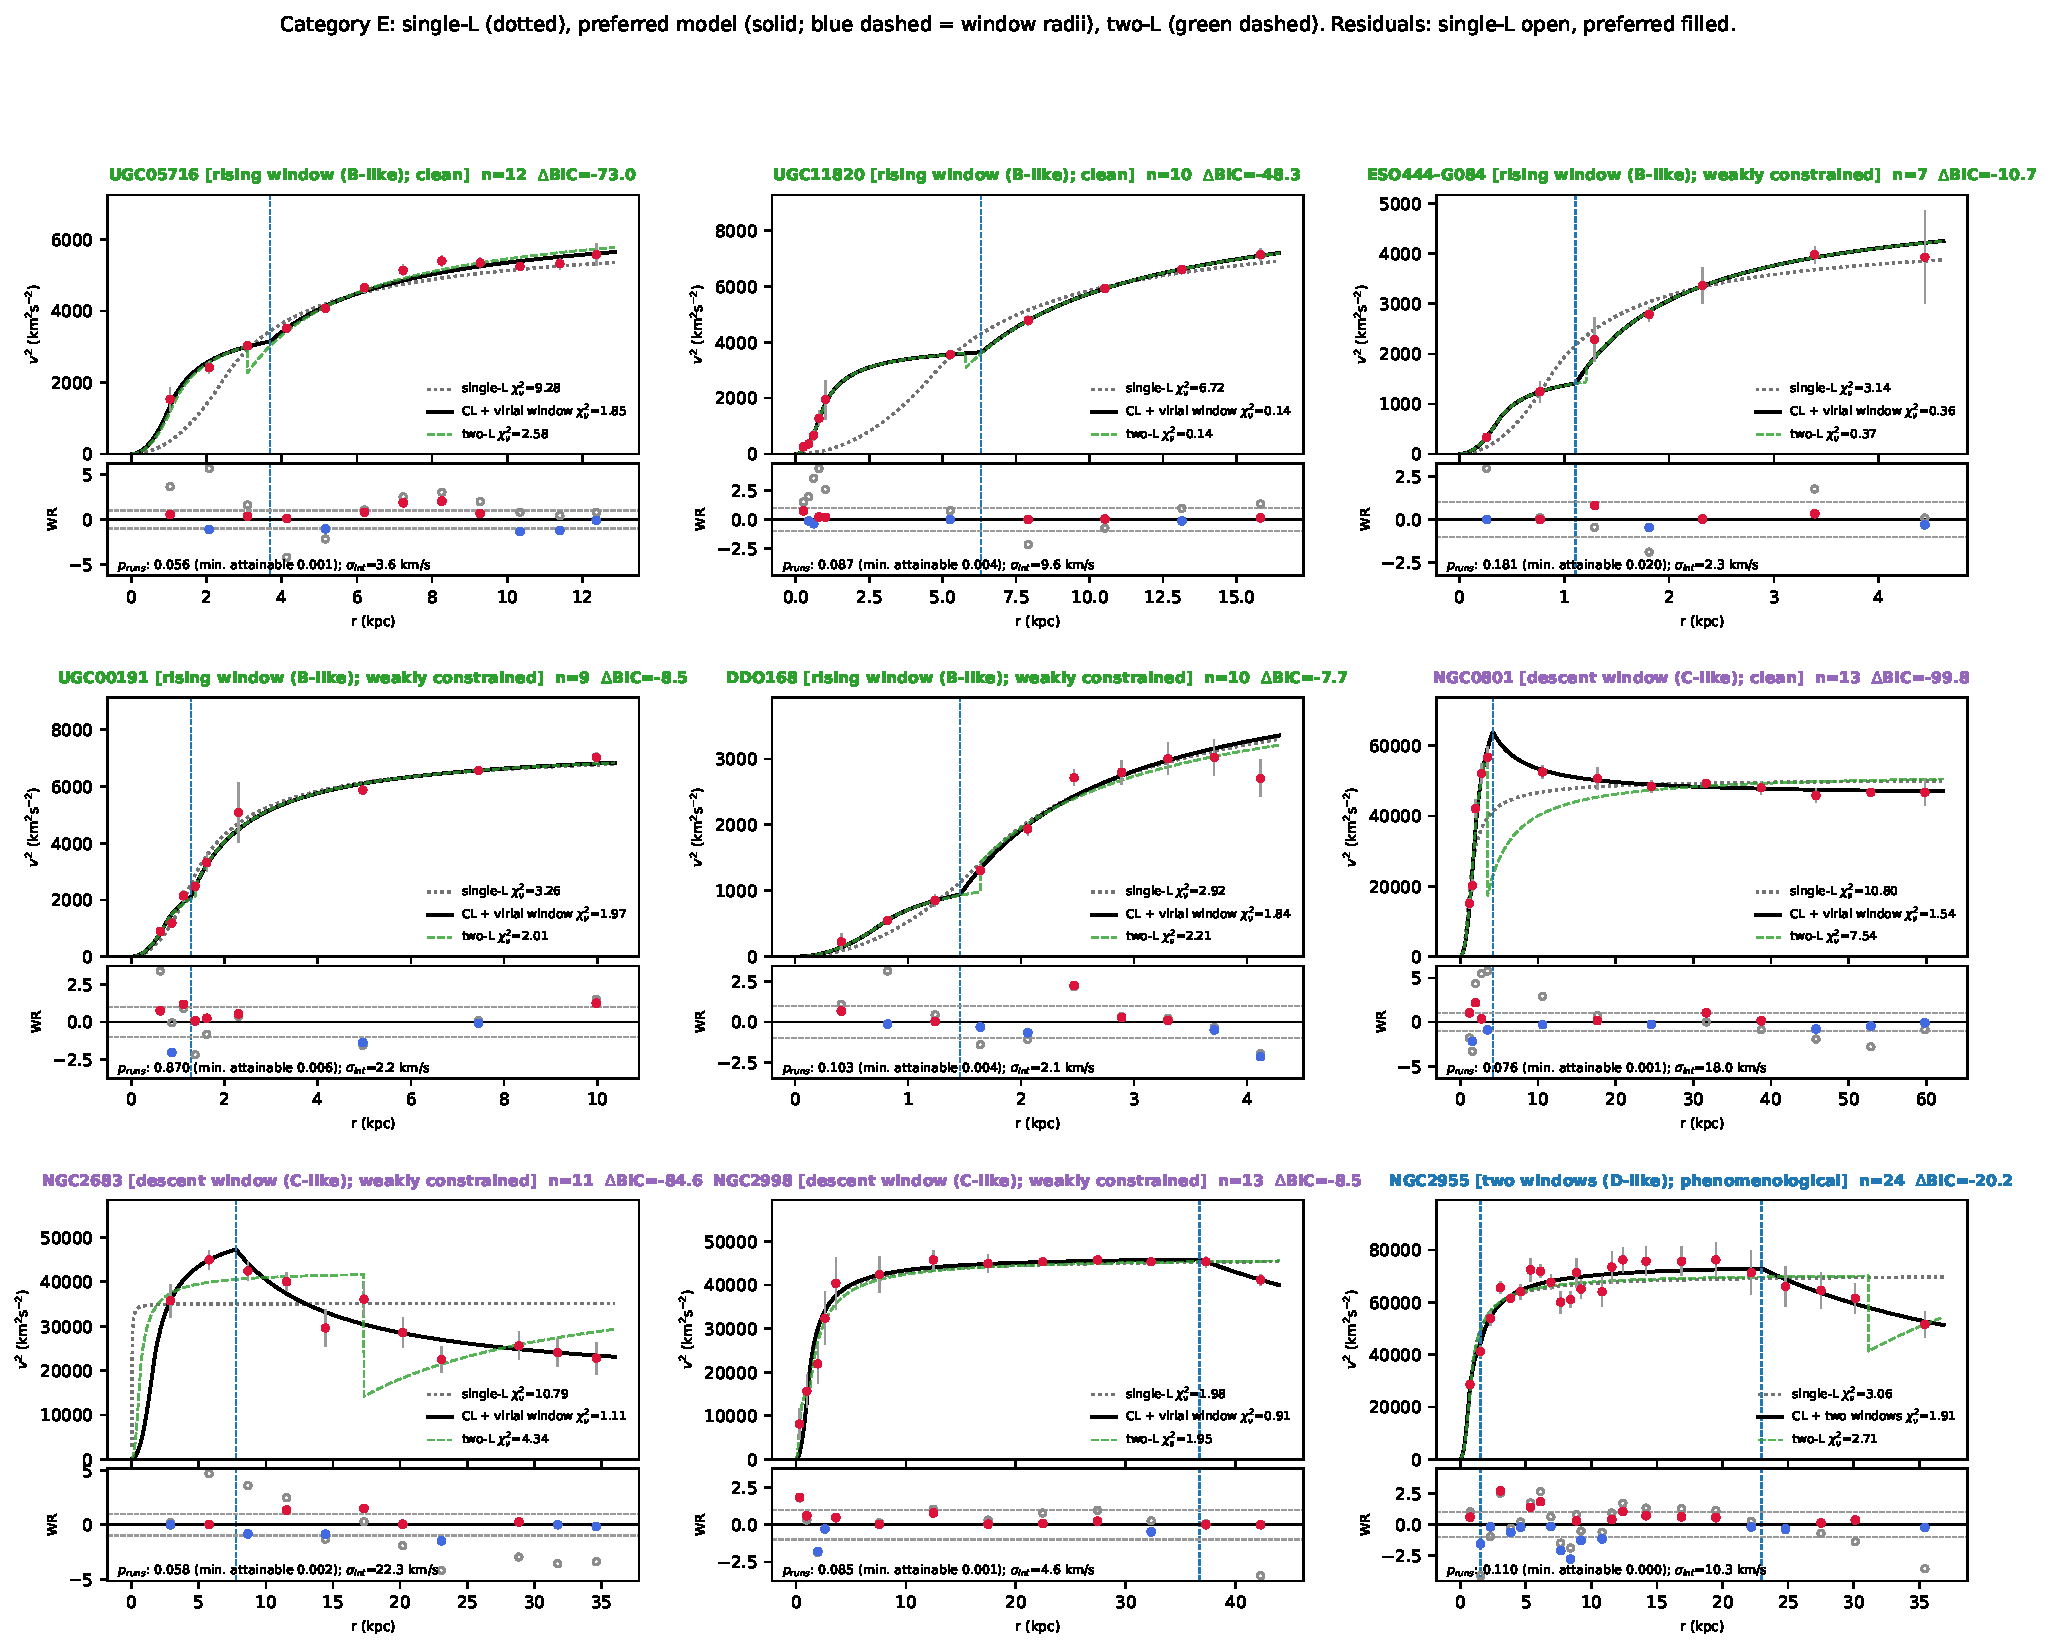
\includepdf[pages=-,landscape=true,scale=0.95]{catE_atlas.pdf}\end{document}